\documentclass[letterpaper]{article}
\usepackage[utf8]{inputenc}
\usepackage[spanish]{babel}
\usepackage{amssymb, amsmath}
\usepackage{graphicx}
\usepackage{lipsum}
\usepackage{wasysym}
\usepackage{dsfont}
\usepackage[margin=1.5cm,
vmargin={2cm,1.3cm},
includefoot]{geometry}
\usepackage{setspace}
\usepackage{subcaption}
\usepackage{tocloft}
\usepackage{upgreek}
\usepackage{amsthm}
\usepackage{graphicx}
\usepackage{paralist}
\usepackage{fancyhdr}
\usepackage{lmodern}
\usepackage{tcolorbox}
\usepackage{color}
\usepackage{tikz}
\tcbuselibrary{skins,breakable}
\pagestyle{fancy}

\renewcommand{\headrulewidth}{0.4pt}
\renewcommand{\footrulewidth}{0.4pt}

\providecommand{\abs}[1]{\lvert#1\rvert}
\providecommand{\norm}[1]{\lVert#1\rVert}														  
\providecommand{\pint}[1]{<#1>}														  
\newcommand{\V}{\mathds{V}}

\newcommand{\W}{\mathds{W}}

\newcommand{\F}{\mathds{F}}

\newcommand{\tq}{ \quad \cdot  \backepsilon \cdot \quad }

\newcommand{\ld}{\lim\limits_{x \to 0^{+}}}

\newcommand{\li}{\lim\limits_{x \to 0^{-}}}

\newcommand{\la}{\lim\limits_{x \to a}}

\newcommand{\R}{\mathds{R}}

\renewcommand{\u}{\vec{u}}

\renewcommand{\v}{\vec{v}}

\newcommand{\Po}{\mathds{P}_2(\mathds{R})}

\renewcommand{\*}{\cdot}

\lhead{}

\chead{Matemáticas para las ciencas aplicadas II}
\rhead{ }

\newcommand{\Iden}{\begin{pmatrix}
		1 & 0 & 0\\
		0 & 1 & 0\\
		0 & 0 & 1 
\end{pmatrix}}
\newcommand{\T}{\begin{pmatrix}
		1 & 3 & 9 \\
		1 & 3 & 4 \\
		0 & 0 & 2 
\end{pmatrix} }

\makeatletter
\renewcommand*\env@matrix[1][*\c@MaxMatrixCols c]{%
	\hskip -\arraycolsep
	\let\@ifnextchar\new@ifnextchar
	\array{#1}}
\makeatother

\newtheorem{theorem}{Teorema}[section]
\newtheorem{corolario}[theorem]{Corolario}
\theoremstyle{definition}
\newtheorem{definition}{Definición}
\begin{document}
	
	\setlength{\unitlength}{1cm}
	\thispagestyle{empty}
	\begin{picture}(19,3)
	\put(-0.5,1.2){
\includegraphics[scale=.20]{unam1.png}}
	\put(16,1){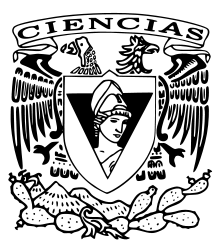
\includegraphics[scale=.29]{fciencias1.png}}
	\end{picture}
	
	\begin{center}
		\vspace{-114pt}
		\textbf{\large Matemáticas para las Ciencias II}\\
		\textbf{ Semestre 2020-2}\\
		Prof. Pedro Porras Flores\\
		Ayud. Irving Hernández Rosas \\
		\textbf{Tarea-examen I}\\[0.2cm]
		\Large \textbf{Apuntes de clase} \footnote{317031326}\\ [0.2cm]
	\end{center}
	\vspace{-10pt}
	\rule{19cm}{0.3mm}
	
\section[Clase 23 de marzo]{Conjuntos abiertos}
\begin{theorem}
	Sean $ \vec{u} $ y $ \vec{v} $ dos vectores en $ \R^3 $ y sea $ \theta  \in \R$, donde $ 0 \leq \theta < \pi $ el ángulo entre ellos, entonces
	\[ <\vec{u}, \vec{v}> = \norm{\vec{u}}\norm{\vec{v}}\cos \theta \]
\end{theorem}
\begin{proof}
	Consideremos el triángulo formado por los vectores $ \vec{u}, \vec{v} $ y $ \vec{u} - \vec{v} $ de la ley de cosenos tenemos 
	\[ \norm{\vec{u}- \vec{v}}^2 = \norm{\vec{u}}^2 + \norm{\vec{v}}^2 - 2 \norm{\vec{u}}\norm{\vec{v}}\cos\theta \label{eq:norma} \tag{ \vernal } \]
	Por otro lado calculemos $ \norm{\vec{u} - \vec{v}}^2 $ esto es
	\begin{align*}
		\norm{\vec{u}- \vec{v}}^2 &= \pint{\u - \v, \u - \v} && \text{Por la definición de $ \norm{ x} $} \\
		\norm{\vec{u}- \vec{v}}^2 &= \pint{\u, \u - \v} + \pint{-\v, \u - \v} \\
		\norm{\vec{u}- \vec{v}}^2 &= \pint{\u, \u - \v} - \pint{-\v, \u - \v} \\
		\norm{\vec{u}- \vec{v}}^2 &= \pint{\u, \u } + \pint{\u, - \v} - \pint{\v, \u} -\pint{\v, \v} \\
		\norm{\vec{u}- \vec{v}}^2 &= \pint{\u, \u } + \pint{\u, - \v} - \pint{\u, \v} +\pint{\v, \v} \\
		\norm{\vec{u}- \vec{v}}^2 &= \norm{\u}^2 + \norm{\v}^2 - 2 \pint{\u, \v} \label{eq:otranorma} \tag{ \ascnode } \\
	\end{align*}
	Comparemos $ \ref{eq:norma} $ con $ \ref{eq:otranorma} $
	\[ -2\norm{\u}\norm{\v}\cos\theta = -2 \pint{\u, \v}  \implies \pint{\u, \v} = \norm{\u}\norm{\v}\cos\theta \quad \forall 0 \leq \theta < \pi \]
\end{proof}
\begin{corolario}[Desigualdad Cauchy-Schwarz]
	Para cualesquiera dos vectores $ \u  $ y $ \v $, se tiene que
	\[ \abs{\pint{\u, \v}} \leq \norm{\u}\norm{\v} \]
	La igualdad se da si y sólo si $ \u $ es múltiplo escalar de $ \v $ o uno de los vectores es 0
\end{corolario}
\begin{proof}
	Supongamos que $ \u $ no es múltiplo escalar  de $ \v $ y viceversa y que además ni $ \u $ ni $ \v $ son cero. Sabemos que\footnotetext[1]{Por nuestro curso de Matemáticas para las ciencias aplicadas I} \[ \abs{\cos} \leq 1 \quad \forall 0 \leq \theta \leq 2 \pi \label{eq:cosacotado} \tag{1} \]
	Por otro lado, sabemos que $ \pint{\u, \v} = \norm{\u}\norm{\v}\cos\theta $, tomando el valor absoluto, tenemos:
	\[ \abs{\pint{\u, \v}} = \norm{\u}\norm{\v}\abs{\cos \theta} \] si multiplicamos a $  (\ref{eq:cosacotado}) $ por $ \norm{\u}\norm{\v} $, entonces tenemos 
	\[ \abs{\pint{\u, \v}} = \norm{\u}\norm{\v}\abs{\cos \theta} \leq (1) \norm{\u}\norm{\v} = \norm{\u} \norm{\v} \]
	Por lo tanto $ \abs{\pint{\u,\v}} \leq \norm{\u}\norm{\v} $
\end{proof}
\newpage
\begin{theorem}[Desigualdad del triángulo]
	Sean $ \u, \v  \in \R^3$, entonces $ \norm{\u + \v} \leq \norm{\u} + \norm{\v} $
\end{theorem}
\begin{proof}
	De la desigualdad de \textit{ Cauchy-Schwarz} tenemos que, 
	\begin{align*}
		\abs{\u, \v} &\leq \norm{\u} \norm{\v} && \text{Por el corolario anterior}\\
		2\abs{\u, \v} &\leq 2\norm{\u} \norm{\v} && \text{como $ 2> 0 $}\\
		2\pint{\u, \v} &\leq 2 \abs{\pint{\u, \v}} && \text{Puesto que } \pint{\u, \v} \leq \abs{\pint{\u, \v}}\\
		2\pint{\u, \v} &\leq 2 \abs{\pint{\u, \v}} \leq  2\norm{\u}\norm{\v}  && \text{Por los dos últimos resltados}\\
		2\pint{\u, \v} &\leq  2\norm{\u}\norm{\v}  && \text{Por transitividad de la desigualdad }\\
		\norm{\u}^2 + \norm{\v}^2 + 2\pint{\u, \v} &\leq \norm{\u}^2 + \norm{\v}^2 + 2\norm{\u}\norm{\v}  && \text{Sumando en ambos lados } \norm{\u}^2 + \norm{\v}^2 \label{eq:desigualdad} \tag{2}\\
	\end{align*}
	Para concluir, observemos que $$ \norm{\u + \v} = \norm{\u}^2 + \norm{\v}^2 + 2 \pint{\u, \v} \label{eq:definicionInterno} \label{3} $$
	Luego, de $ (\ref{eq:desigualdad}), (1) $ tenemos: 
	$ \norm{\u + \v} \leq \norm{\u}^2 + \norm{\v}^2 + 2 \norm{\u} \norm{\v} $, ahora tenemos 
	\begin{align*}
	\norm{\u+ \v}^2 & \leq (\norm{\u} + \norm{v})^2 && \text{factorizando el trinomio cuadrado pefecto}\\
	\norm{\u+ \v} & \leq \norm{\u} + \norm{v} && \text{Tomando la raíz cuadrada}
	\end{align*}
\end{proof}
\begin{corolario}
	Sean $ \u, \v \in \R^3 $, muestre que $ \norm{\u - \v} \geq \abs{\norm{\u} - \norm{\v}} $
\end{corolario}
\section{Bola abierta}
\begin{definition}[Bola abierta]
	Sea $ \vec{x_0} $ y sea $ r \in \R^+ $, la bola de radio $ r $ y centro en $ \vec{x_0} $ es definida por el conjunto de todos los punros $ \vec{x} $ tal que $ \norm{\vec{x} - \vec{x_0}} < r $.\\
	Este conjunto es denotado como $ Br(\vec{x_0}) $, es el conjunto de todos los puntos $ \vec{x} \in \R^n $ cuya distancia de $ \vec{x_0} $ es menor que $ r $
	\[ Br(\vec{x_0}) = \{  \norm{\vec{x} - \vec{x_0}} < r \quad | \quad \vec{x}, \vec{x_0} \in \R^n \quad r > 0 \} \]
\end{definition}
%%%%%%%%%%%%%%%%%%%%%%%%%%%%%%%%%%%%%%%
%
%		EJEMPLOS DE BOLAS AABIERTAS
%
%%%%%%%%%%%%%%%%%%%%%%%%%%%%%%%%%%%%%%%
\begin{definition}[Conjunto abierto]
	Sea $ U \subset \R^n $. Decimos que $ U $ es un conjunto abierto si para cada $ \vec{x_0} \in U $, existe algún $ r > 0 $ tal que $ Br(\vec{x_0}) $ está totalmente contenida en $ U $, $ Br(\vec{x_0}) \subseteq U $
\end{definition}
%%%%%%%%%%%%%%%%%%%%%%%%%%%%%%%%%%%%%%%
%
%		EJEMPLOS QUE PORRAS PUSO EN EL PLANO Y UN SUBVONJUNTO
%
%%%%%%%%%%%%%%%%%%%%%%%%%%%%%%%%%%%%%%%
\begin{theorem}
	Para cada $ \vec{x_0} \in \R^n $ y $ r >0 $, $ Br(\vec{x_0})  $ es un conjunto abierto
\end{theorem}
\begin{proof}
	Para mostrar que $ Br(\vec{x_0}) $ es abierto, debemos mostrar que para cualquier punto $ \vec{x} \in Br(\vec{x_0})  $ podemos dar una bola con centro en $ \vec{x} $ y algún radio, además que dicha bola esté totalmente contenida en $ Br(\vec{x_0}) $, a continuación mostraremos un bosquejo que ayuda a la prueba\\

Observemos que el radio para la bola con centro en $ \vec{x} $, debe ser \[ s = r - \norm{\vec{x} - \vec{x_0}} \label{eq:radio} \tag{1} \]
Ahora sólo mostraremos que $ Br(\vec{x}) \subset Br(\vec{x_0}) $. Para esto debemos mostrar que para cualquier $ \vec{y} \in Br(\vec{x}) $, entonces $ \vec{y} \in Br(\vec{x_0}) $. Esto es \[ \norm{ \vec{y} - \vec{x} } < s \implies \norm{\vec{y} - \vec{x_0}} < s \] Hagamos una observación, como $ \vec{y} \in Br(\vec{x}) $ entonces \[ \norm{ \vec{y} - \vec{x} } < s \label{eq:bola} \tag{2} \] esto anterior, por la definición de bola.\\
	
	En resumen, debemos de mostrar que $ \norm{\vec{y} - \vec{x_0} } < r $, para ello consideremos:
	\begin{align*}
	\norm{\vec{y} - \vec{x_0}} &= \norm{\vec{y} + \vec{0} - \vec{x_0}} & \text{Sumando el neutro aditivo}\\
	\norm{\vec{y} - \vec{x_0}} &= \norm{\vec{y} + \vec{x} - \vec{x} - \vec{x_0}} & \text{Por definición del neutro aditivo}\\
	\norm{\vec{y} - \vec{x_0}} &= \norm{(\vec{y} - \vec{x}) + (\vec{x} - \vec{x_0})} & \text{Por definición del neutro aditivo}\\
	\norm{\vec{y} - \vec{x_0}} &= \norm{(\vec{y} - \vec{x}) + (\vec{x} - \vec{x_0})} \leq \norm{\vec{y} - \vec{x}} + \norm{ \vec{x} - \vec{x_0} } & \text{Por la desigualdad del triángulo}\\
	\norm{\vec{y} - \vec{x_0}} &= \norm{(\vec{y} - \vec{x}) + (\vec{x} - \vec{x_0})} \leq \norm{\vec{y} - \vec{x}} + \norm{ \vec{x} - \vec{x_0} } < s + \norm{\vec{x} + \vec{x_0}} & \text{Por la observación \ref{eq:bola} } \norm{ \vec{y} - \vec{x} } < s 
	\end{align*}
	Finalmente por $ (\ref{eq:radio}) $ \[ \norm{\vec{y} - \vec{x_0}}< r \]
\end{proof}
\section*{Ejemplo}
Mostrar $ A = \{ (x,y) \in \R^2 | x > 0 \} $ es un conjunto abierto
\begin{proof}
	Sean $(x,y) \in A $ y $ r > 0 $, por mostrar que $ Br(x,y)  \subset A$. Observamos que la bola más grande que podemos dar con centro en $ (x,y) $ es la que tenga un radio $ r = x $, pues como $ (x,y) \in A $, entonces $ x >0 $.\\
	
	Ahora queremos mostrar que si tomamos $ (x_1,y_1) \in Br(x,y) $ entonces $ (x_1,y_1) \in A $.\\
	
	Si $ (x_1,y_1) \in Br(x,y) $, entonces
	\begin{align*}
	\abs{x_1 - x} &= \sqrt{(x_1 - x)^2} && \text{Por definición de valor absoluto}\\
	\abs{x_1 - x} &= \sqrt{(x_1 - x)^2} \leq \sqrt{(x_1 - x)^2 + (y_1 - y)^2} < r = x && \text{Por construcción}\\
	\abs{x_1 - x} & < x && \text{Transitividad de la desigualdad}\\
	-x &< x_1 - x < x && \text{Propiedad del valor absoluto}\\
	0 &< x_1  < 2x && \text{Sumando en todos lados }x\\
	0 &< x_1  && \text{Tomando sólo esa parte de la desigualdad}\\
	\end{align*}
	\[ 0 < x_1 \implies (x_1,y_1) \in A \implies Br(x,y) \subset A \]
	\begin{center}
		$ \therefore $ A es abierto
	\end{center} 
\end{proof}
	El concepto de bola en $ \R^n $ permite extender el concepto de vecidad qe teníamos en $ \R $, la cual fue fundamental para definir conceptos como límite y continiudad
	\section{Frontera}
	A continuación introducimos el concepto de frontera.
	\begin{definition}[Punto frontera]
		Sea $ A \subset \R^n$. Un punto $ \vec{x} \in \R^n $, es llamado punto frontera de $ A $ si para cada vecindad de $ \vec{x} $, ésta contiene al menos un punto de $ A $ y punto que no está en $ A $, la frontera de $ A $ son todos sus puntos frontera.
	\end{definition}
\section*{Ejemplo}
Sea $ A = (a,b)  \in \R$, entonces los puntos frontera de A son $ a  $ y $ b $.
%%%%%%%%%%%%%%%%%%%%%%%%%%%%%%%%%%%%%%%%%
%	Aquí ponemos una linea recta con intervalos abiertos
%%%%%%%%%%%%%%%%%%%%%%%%%%%%%%%%%%%%%%%%%

Mostremos que $ a $ es un punto frontera, para esto observemos que la bola más grande que podemos dar es aquella cuyo radio sea $ \abs{b -a} $.Sea 
\[ Br(a) = \{ \abs{x -a} < r | r < \abs{b-a} \} \] y como $ a<b $, entonces $ 0 < b -a $ por lo que $ \abs{b-a} = b-a >0 $
\[ Br(a)  = \{ -r < x-a < r | r < b-a \} \]
Por otra parte, observemos lo siguiente
\[ r < b-a \implies -r > -(b-a) \implies -r > a-b \]
Así obtenemos que
\[  -r > a-b \implies Br(a) = \{ a-b < x-a < b-a | a<b \} \]
\[ Br(a) = \{ a-b < x-a < b-a | a<b \} \implies Br(a) = \{ 2a-b < x < b \} \]Observemos lo siguiente, como $ a< b  \implies a-b < 0 \implies a +a -b < a  \implies 2a - b < a$. Por lotanto, hay $ x $ tal que $ 2a-b < x < a $, es decir, $ x $ es un punto que no está en $ A $ y por otro lado como $ x<b $ también hay al menos un punto que sí lo está, por lo tanto $ a $ es punto frontera. Análogo  para $ b $.

Las pruebas para las siguientes fronteras las hicimos en clase\\


b) Sea $ A  = Dr(x_0,y_0)$, un disco en el plano (Bola en $ \R^2 $)\\


c) Sea $ A = \{ (x,y) \in \R^2 | x > 0\} $. Encontrar la frontera de $ A $ consiste de todos los puntos del eje $ y $
\section{Límites}
Recordemos la definición de límite de funciones de $ \R $ en $ \R $.\\

Sea $ f: I\subset  \R \to \R $, $ L $ es el límite de $ f $ en $ a $ si para cada $ \epsilon > 0, \quad \exists \delta > 0 $, tal que $ \forall x \in Dom(f) $, si $ 0 < \abs{x - a} < \delta $, entonces $ \abs{f(x) - L} < \epsilon $ lo que denotamos como
\[ \lim\limits_{x \to a}f(x) = L \]
\begin{definition}[Límite de funciones de $ \R^n $ en $ \R^m $]
	Sean $ f: A \subset \R^n \to  \R^m $ y $ \vec{x_0} \in A $ un punto de acumulación de $ A $. Entonces se dice que el límite de $ f(\vec{x}) $, cuando $ \vec{x} $ tiende a $ \vec{x_0} $, es $ \vec{l} \in \R^m $ y se denota:
	\[ \lim\limits_{\vec{x} \to \vec{x_0}}f(\vec{x}) = \vec{l} \quad \text{ o } f(\vec{x}) \to \vec{l}, \text{ si } \forall \epsilon > 0, \exists \delta > 0 \text{ tal que } \vec{x} \to \vec{x_0} \]
	$ 0 < \norm{\vec{x} - \vec{x_0}} < \delta $ y $ \vec{x} \in A $, entonces $ \norm{f(\vec{x}) - \vec{l}} < \epsilon $. Esto es equivalente a: Si $ \forall \epsilon > 0, \quad \exists \delta > 0  $ tal que \[ f([B_\delta(\vec{x_0})\cap A]\backslash\{ \vec{x_0} \}) \subseteq B_\epsilon(\vec{l}) \]
\end{definition}
\begin{figure}[h]
	\centering
	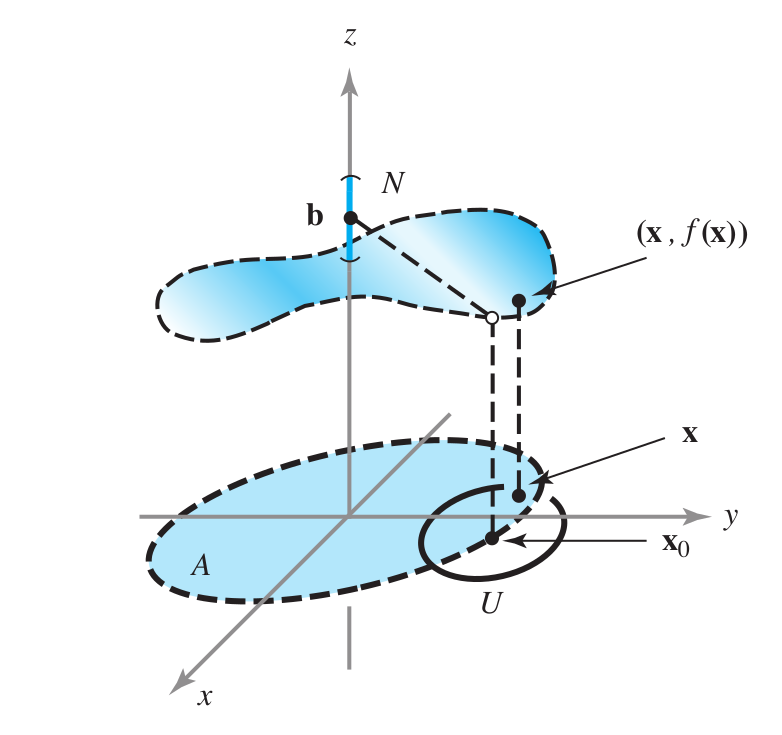
\includegraphics[width=0.3\textwidth]{img/limite}
	\caption{Límite en términos de vecidades}
\end{figure}
\section{Propiedades de límites}
\begin{theorem}[ Unicidad de límites]
	Si $ \lim\limits_{\vec{x} \to \vec{x_0}}f(\vec{x}) = \vec{l_1} $ y $ \lim\limits_{\vec{x} \to \vec{x_0}}f(\vec{x}) = \vec{l_2} $, entonces $ \vec{l_1} = \vec{l_2} $
\end{theorem}
\begin{proof}
	Para mostrar el teorema, veremos que $ \norm{\vec{l_1} - \vec{l_2}} = 0 $, observemos $$ 0 \leq \norm{\vec{l_1} - \vec{l_2}} = \norm{\vec{l_1} - \vec{l_2} + 0} = \norm{\vec{l_1} - \vec{l_2} + f(\vec{x}) - f (\vec{x})}  $$ Agrupando $ 0 \leq \norm{\vec{l_1} - \vec{l_2}} = \norm{(\vec{l_1} - f(\vec{x})) + (f(\vec{x}) - \vec{l_2})} $\\
	
	\noindent Usando la desigualdad del triángulo,entonces
	\[ 0 \leq \norm{\vec{l_1} - \vec{l_2}  }  \leq \norm{ \vec{l_1} - f(\vec{x}) } + \norm{f(\vec{x}) - \vec{l_2}}  \] 
	Pero por hipótesis $ \lim\limits_{\vec{x} \to \vec{x_0}}f(\vec{x}) = \vec{l_1} $ y $ \lim\limits_{\vec{x} \to \vec{x_0}}f(\vec{x}) = \vec{l_2} $\\

	\noindent Entonces $ \norm{ \vec{l_1} - f(\vec{x}) } \to 0 $ y $ \norm{f(\vec{x}) - \vec{l_1}} \to 0  $, entonces
	\[ 0 \leq \norm{\vec{l_1} - \vec{l_2}} \leq 0  \] por lo tanto $ \vec{l_1} - \vec{l_2}  = 0 \implies \vec{l_1} = \vec{l_2} $
\end{proof}
\section*{Ejemplos}
\end{document}